\section{Project Setup}
The following components were present in the lab:

\begin{itemize}
    \item Model Car: The model car has three servos for the brakes, one servo for steering and an engine for acceleration. All of these components are controlled via a servo controller board.
    
    \item Servo Controller Board: The servo controller board is a \textit{polulu maestro servo controller board} which is attached to a Raspberry Pi via a usb-to-uart bridge.

    \item Raspberry Pi: The Raspberry Pi is responsible for sending control commands to the servo controller board. It receives its input data from a PandaBoard via a mqtt topic to which it is subscribed. The Raspberry Pi runs Genode with FiascoOC.

    \item PandaBoard: Besides the Raspberry Pi, the PandaBoard is the second ECU in the model car. It also runs Genode with FiascoOC. The task is to receive data from a simulation, transform the data into concrete servo values and send them via mqtt to the Raspberry Pi.
\end{itemize}

An image of the model car is shown in figure \ref{fig:model}.

\begin{figure}[h]
    \centering
    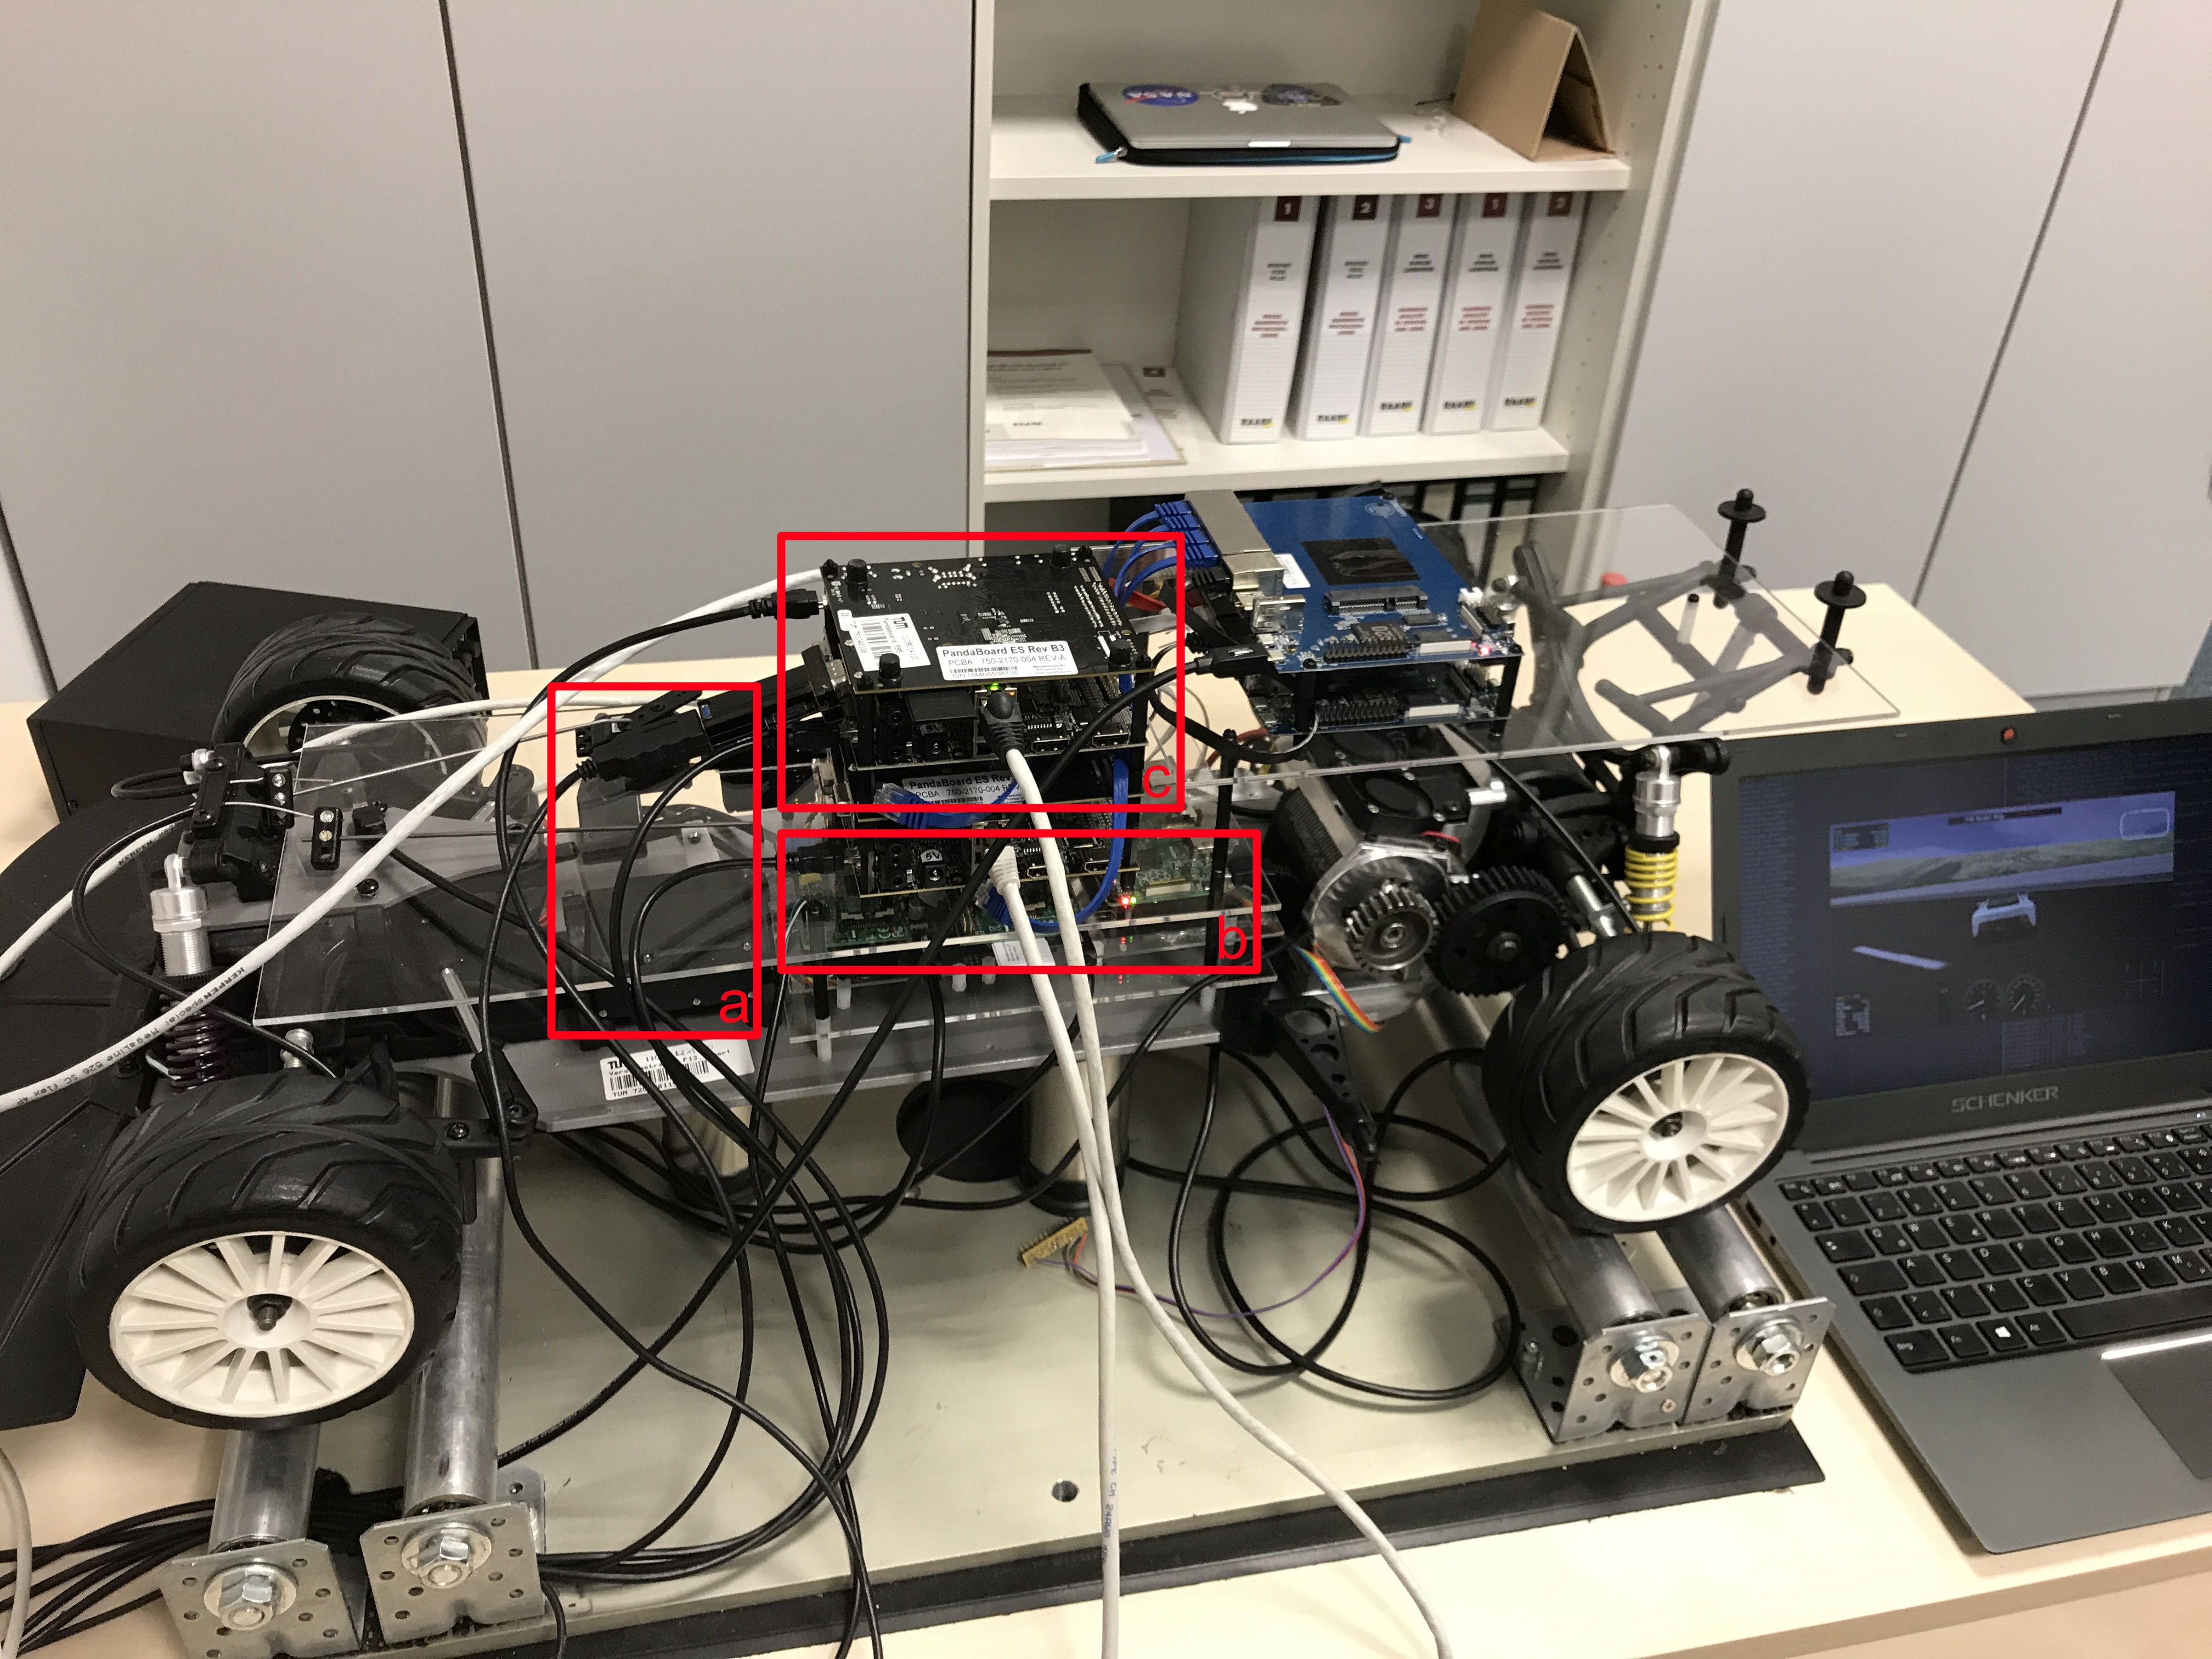
\includegraphics[width=0.70\linewidth]{images/model}
    \caption{Model Car}
    \label{fig:model}
\end{figure}



\section{Source Code Structure}
\paragraph{old}
In the old folder source code for linux and scripts for working with the pololu maestro servo controller board can be found, which were used during development.

\paragraph{run}
In the run folder the run files for the ecu(car\_panda) and the servo controller(car\_rpi) are placed.

\paragraph{include}
In the include directory the header files for the servo and the controller component are split up into their respective folders.

\paragraph{src}
In the source(src) directory all source files used can be found. In the subdirectory mqtt is a class that implements the mosquitto interface, which is used in the panda and the rpi targets. Each of the two targets is further split up into its main component and a secondary component including each a target.mk for the build process and the actual \CC-source file.

\section{Application Programming Interfaces}

